\documentclass[12pt,oneside]{amsart}
\usepackage{amsmath}
\usepackage{lipsum}
\usepackage{multicol}
\usepackage{caption}

\linespread{1}

% Adjust page margins and spacing
\setlength{\topmargin}{-0.5in}       % reduce top margin
\setlength{\textheight}{9.5in}       % increase usable vertical space
\setlength{\oddsidemargin}{0.1in}    % reduce side margins
\setlength{\evensidemargin}{0.1in}   % ensure consistency
\setlength{\textwidth}{6.3in}        % increase usable horizontal space

% Caption settings
\captionsetup{font=scriptsize}
\captionsetup[table]{skip=10pt}

%-------Packages---------
\usepackage{amssymb,amsfonts}
\usepackage[all,arc]{xy}
\usepackage{enumerate}
\usepackage{mathrsfs}
\usepackage{graphicx}
\usepackage{epstopdf}
\usepackage{listings}
\usepackage{appendix}
\usepackage{listings}
\usepackage{placeins}
\usepackage{booktabs}
\usepackage{tabularx}


%--------Theorem Environments--------
%theoremstyle{plain} --- default
\newtheorem{thm}{Theorem}[section]
\newtheorem{cor}[thm]{Corollary}
\newtheorem{prop}[thm]{Proposition}
\newtheorem{lem}[thm]{Lemma}
\newtheorem{conj}[thm]{Conjecture}
\newtheorem{quest}[thm]{Question}

\theoremstyle{definition}
\newtheorem{defn}[thm]{Definition}
\newtheorem{defns}[thm]{Definitions}
\newtheorem{con}[thm]{Construction}
\newtheorem{exmp}[thm]{Example}
\newtheorem{exmps}[thm]{Examples}
\newtheorem{notn}[thm]{Notation}
\newtheorem{notns}[thm]{Notations}
\newtheorem{addm}[thm]{Addendum}
\newtheorem{exer}[thm]{Exercise}

\theoremstyle{remark}
\newtheorem{rem}[thm]{Remark}
\newtheorem{rems}[thm]{Remarks}
\newtheorem{warn}[thm]{Warning}
\newtheorem{sch}[thm]{Scholium}
\newcommand{\be}{\begin{equation}}
\newcommand{\ee}{\end{equation}}
\makeatletter
\let\c@equation\c@thm
\makeatother
\numberwithin{equation}{section}

\usepackage[style=apa,sortcites=true,sorting=nyt,backend=biber,natbib=true]{biblatex}
%bibliographystyle{unsrtnat}
\addbibresource{Reference/reference.bib}
%%%%%%%%%%%%%%%%%%%%%%%%%%%%%%%%%%%%%%%%%%%%%%%%%%%%%%%%%%%%%%%%%%%%%%%%%%%%%%%%%
% your title/author/date information go here
%--------Meta Data: Fill in your info------


\title{Variable Selection in Risk Difference Estimation}

\author{Xuan Li}

\date{Feb 25, 2025}

\begin{document}

\begin{abstract}
    This report serves as a qualifying paper for the UBC Statistics PhD program, providing a comprehensive summary of the paper “Variable Selection When Estimating Effects in External Target Populations” \citep{qp}. The original paper shows that, to generalize risk difference estimates from a study population to a target population, one should include effect measure modifiers (EMMs) that differ between the populations; while adding non-EMMs differing between the populations might reduce precision, it does not amplify bias. Through simulations, we show that accounting for critical EMMs—both with and without interaction terms—consistently yields unbiased RD estimates, even when treatment assignment is not random. Moreover, we find that including interactions improves precision slightly but does not necessarily improve bias under the current experimental setup, suggesting potential areas for further methodological refinement.
\end{abstract}
\maketitle
\tableofcontents

%%%%%%%%%%%%%%%%%%%%%%%%%%%%%%%%%%%%%%%%%%%%%%%%%%%%%%%%%%%%%%%%%%%%%%%%%%%%%%%%%section 1


\section{Introduction}

\subsection{Background and Motivation}

Causal inference often requires estimating the treatment effects of study populations and generalizing them to target populations. One commonly used measure is the \textbf{risk difference (RD)}, which quantifies the difference in outcome probability between exposed and unexposed groups:
\begin{equation}
    RD = P(Y = 1 \mid X = 1) - P(Y = 1 \mid X = 0).
\end{equation}
In an ideal scenario, we can estimate RD using a study sample and apply it to a target population. However, differences in covariate distributions between study and target populations can lead to biased estimates.

A key challenge is selecting the appropriate covariates when modeling RD. An effect measure modifier (EMM) is a variable that changes the relationship between exposure and outcome \citep{rd}, in other words, it affects how exposure influences outcome. Non-effect measure modifiers (non-EMMs) do not modify the relationship between the exposure and the outcome, but can still affect the outcome independently. Understanding how different sets of variables influence model estimates in an external target population can enhance generalizability and improve the accuracy of effect estimation. 

\subsection{Summary of the Original Paper}
The paper \textit{``Variable Selection When Estimating Effects in External Target Populations''} primarily examines how covariate selection affects RD estimation when transporting causal effects from a study population to an external target population. The authors explore different modeling approaches, including \textbf{outcome modeling (OM)} and \textbf{inverse odds weighting (IOW)}, to assess their impact on bias and precision.

The authors examined various covariate sets and concluded that \textbf{effect measure modifiers (EMMs) differing across study and target populations} must be included—omitting them increases bias in transporting the RD to the target population. Meanwhile, \textbf{adding non-EMMs that differ} across populations inflates variance but does \textbf{not} amplify bias. These results challenge common intuitions from the internal validity setting and the discrepancy is explained by two main reasons from the authors: 
\begin{itemize}
    \item \textbf{Internal vs. External Validity Focus.} In \textbf{internal validity} (e.g., within a single study), one aims for conditional exchangeability between treated and untreated individuals, so adding strong outcome predictors (regardless of whether they modify the effect) can boost efficiency \citep{internal}. In \textbf{external validity}, the key is conditional exchangeability between \textit{populations}, so the real analog of “outcome predictors” are the \textbf{EMMs}. Non-EMMs don’t mitigate external bias and merely increase variance.
    \item \textbf{Instrument-Like Variables vs. Non-EMMs}. In internal validity, instruments (variables related to the exposure) can amplify bias if unmeasured confounders are present \citep{instrument}. However, in external validity, the situation differs since the role of these variables differs. Here, non-EMMs that vary between study and target populations primarily reflect \textbf{sampling mechanisms} rather than confounding structures. As a result, we don’t observe bias amplification from non-EMMs in external validity as we do with instruments in internal validity.
\end{itemize}

\subsection{Empirical Simulation in the Paper}
The authors consider six covariates $Z$'s in the original paper for simulation. The six covariates differ in two main aspects: (1) their distributions across the study and target populations, and (2) whether they affect the outcome $Y$ and/or modify the effect of $X$ on $Y$ (i.e., whether they are effect modifiers). 

The study focuses on binary treatment \textit{X} and binary outcome \textit{Y}. The true underlying process (DGP) of $P(Y|X, \textbf{Z}) $ with interaction terms of $X$ and $Z$'s is: $$P(Y|X, \textbf{Z}) = 0.1 + 0.1 \times X + 0.1 \times Z_2 + 0.1 \times Z_3 + 0.1\times Z_5 + 0.1 \times Z_6 + 0.1 \times X\times  Z_3 + 0.1 \times X \times Z_6,$$ where $Z$'s represent other covariates besides treatment assignment $X$. In the paper's simulation set-up, the treatment assignment $X$ is random in both the target and the study data generation process. Note that \textbf{$Z_3, Z_6$ are EMMs}, as they interact with $X$ in the DGP. \textbf{$Z_2, Z_5$ are non-EMMs}, affecting $Y$ but not modifying the effect of $X$ on $Y$. $Z_1$ and $Z_4$ are variables that neither affect $Y$ nor affect how $X$ influence $Y$. In the setup, $Z_1$, $Z_2$ and $Z_3$ are distributed in the same way across the study and target populations, while $Z_4$, $Z_5$ and $Z_6$ are distributed differently between the two populations. 

The authors evaluate different linear model specifications for RD estimation under both \textbf{outcome modeling (OM)} and \textbf{inverse odds weighting (IOW)}. Below is a summary of key models used in their analysis in Table \ref{tab:model}. Each of these models is applied in both the OM and IOW approaches. For the Outcome Modeling (OM) approach, linear models without interaction terms are fitted to stratified $X$ in the study data and used to predict RD in the target population. For the inverse odds weighting (IOW) approach, linear weights are assigned to account for the different distributions of covariates between the study and target populations. 

\begin{table}[h]
    \centering
    \begin{tabular}{lll}
        \toprule
        \textbf{Model} & \textbf{Specification} & \textbf{Covariates Included} \\
        \midrule
        \( M_{\text{crude}} \) & Crude Model & \( X \) only \\
        \( M_1 \) & Non-EMM \( Z_1 \) only & \( X, Z_1 \) \\
        
        \( M_2 \) & Non-EMM \( Z_2 \) only & \( X, Z_2 \) \\
        \( M_3 \) & EMM \( Z_3 \) only & \( X, Z_3 \) \\  
        \vdots & \vdots & \vdots\\
        
        \( M_{1,6} \) & Non-EMM \( Z_1 \) + EMM \( Z_6 \) & \( X, Z_1, Z_6 \) \\
        \( M_{2,6} \) & Non-EMM \( Z_2 \) + EMM \( Z_6 \) & \( X, Z_2, Z_6 \) \\
        \( M_{3,6} \) & EMM \( Z_3 \) + EMM \( Z_6 \) & \( X, Z_3, Z_6 \) \\
        \vdots & \vdots & \vdots\\

        \bottomrule
    \end{tabular}
    \caption{Models Tested in the Paper}
    \label{tab:model}
\end{table}

In the set-up, 10,000 data are generated in study population and 10,000 data are generated in target population. The authors conduct 20,000 simulations in total. Additionaly, the authors also perform sensitivity analyzes in different study-target sizes and risk metrics. 

\subsection{Simulation Results}
Empirically, the study finds that including non-EMMs does not amplify bias but reduces precision in both the OM and IOW approaches. The minimally sufficient adjustment set includes only \( Z_6 \), the EMM that distributes differently between the study and target populations. Including non-EMMs identical between study and target has no effect, while including non-EMMs differing between populations besides the key EMM (such as including both $Z_1$ and $Z_6$) increases the empirical standard error (or standard deviation of the RD estimates across 20000 simulations) compared to only including $Z_6$. When $Z_6$ is omitted, all estimates are biased (RD = 0.170), but adjusting for additional covariates does not amplify this bias compared to the crude model. Outcome modeling (OM) suffers less precision loss than inverse odds weighting (IOW). The sensitivity analyzes further confirm these findings. 

In summary, the paper suggests that including only EMMs that differ between study and target is sufficient to obtain unbiased RD estimates. We should avoid adjusting for Non-EMMs that differ across populations. 


\subsection{Limitations}
Although the authors provide valuable empirical results, their study has several limitations. First, all models they tested are in fact \textbf{misspecified} because none includes any interaction term \( X\times Z_3 \) or \( X\times Z_6 \), which are present in the true data-generating process (DGP). This means that all RD estimates come from \textbf{"incorrectly"} specified models, raising the question of how meaningful the comparisons between these models truly are and whether similar patterns would emerge if the models correctly accounted for interaction effects. Second, the simulation setup assumes that treatment \(X\) is randomly assigned in the target population, an assumption that often does not hold in real-world applications. In practice, exposure is typically influenced by the underlying covariates, which introduces potential selection bias that the study does not account for. Third, the study lacks a theoretical derivation of the bias and variance properties of RD estimators. Although empirical findings suggest that including non-EMMs increases variance without introducing bias, there is no formal mathematical justification supporting this conclusion.

Other limitations include the use of a \textbf{linear probability model} instead of the more commonly used logistic model for binary outcomes, which may lead to less accurate probability estimates, especially when outcome probabilities are near $0$ or $1$. Additionally, the study does not incorporate confounding effects, assuming no unmeasured common causes of both \(X\) and \(Y\). In many practical settings, unmeasured confounding can bias causal effect estimates, making it an important factor to consider in generalizing RD estimates. Given these limitations, our report aims to further investigate several of these issues and assess their implications for RD estimation in external validity settings.


\subsection{Exploring the Theoretical Approach}
While the main findings of the paper rely on empirical simulations, we try to explore a simplified theoretical framework to understand why including non-EMMs does not increase bias but does decrease precision. Consider a simplified version of the DGP for $Y$ given exposure \( X \) and covariates \( Z_1, Z_2 \) used in the original paper:
\begin{equation}
    P(Y = 1 \mid X, Z_1, Z_2) = \beta_0 + \beta_1 \times X + \beta_2 \times Z_1 + \beta_3 \times X \times Z_2
\end{equation}
where \( Z_1 \) is a non-EMM, and \( Z_2 \) is an EMM. In this case, the true RD, defined as $RD = P(Y = 1 \mid X = 1) - P(Y = 1 \mid X = 0)$ simplifies to:
\begin{equation}
    RD = \beta_1 + \beta_3 Z_2.
\end{equation}

However, as done in the simulation from the original paper, we do not fit the true model; instead, we fit \textbf{misspecified models} that omit interaction terms. We explore the bias and variance of RD under three model specifications.

\textbf{Model 1}: Suppose we fit a linear model that includes \( X \) and \( Z_1 \), but omits \( Z_2 \) and its interaction with \( X \):
\begin{equation}
    \hat{P}(Y = 1 \mid X, Z_1) = \hat{\beta}_0 + \hat{\beta}_1 X + \hat{\beta}_2 Z_1.
\end{equation}
The \textbf{estimated RD} from this model is:
\begin{equation}
    \hat{RD} = \hat{\beta}_1,
\end{equation}
The \textbf{bias} of estimated RD is therefore:
\begin{equation}
    \text{Bias}(\hat{RD}) = (\beta_1 - \hat{\beta}_1) + \beta_3 E[Z_2].
\end{equation}
The term \( \beta_1 - \hat{\beta}_1 \) arises from \textbf{estimation error} and the term \( \beta_3 E[Z_2] \) is the bias introduced by omitting the interaction term \( X \times Z_2 \). The variance of estimated RD in this case is given by:
\begin{equation}
    \text{Var}(\hat{RD}) = \left[(X^T X)^{-1}\right]_{11} \sigma^2.
\end{equation}
where \( \sigma^2 \) is the residual variance and $\left[(X^T X)^{-1}\right]_{11}$ is the entry in the inverse matrix \( (X^T X)^{-1} \) corresponding to \( \beta_1 \)
\\

\textbf{Model 2}: Now consider an alternative model that includes \( X \) and \( Z_2 \), but omits \( Z_1 \):
\begin{equation}
    \hat{P}(Y = 1 \mid X, Z_2) = \hat{\beta}_0^* + \hat{\beta}_1^* X + \hat{\beta}_3^* Z_2.
\end{equation}
Here, the \textbf{estimated RD} is:
\begin{equation}
    \hat{RD}^* = \hat{\beta}_1^*.
\end{equation}
The \textbf{bias} of estimated RD in this model is:
\begin{equation}
    \text{Bias}(\hat{RD}^*) = (\beta_1 - \hat{\beta}_1^*) + \beta_3 E[Z_2].
\end{equation}
The term \( \beta_1 - \hat{\beta}_1^* \) is again due to \textbf{estimation error} and the term \( \beta_3 \) is due to omitting the interaction term \( X \times Z_2 \). The \textbf{variance} of estimated RD in this case is:
\begin{equation}
    \text{Var}(\hat{RD}^*) = \left[(X^T X)^{-1}\right]_{11}^* \sigma^2.
\end{equation}

\textbf{Model 3}: Now consider another  model that includes \( X \), \( Z_1 \) and \( Z_2 \) :
\begin{equation}
    \hat{P}(Y = 1 \mid X, Z_2) = \hat{\beta}_0^\# + \hat{\beta}_1^\# X + \hat{\beta}_2^\# Z_1 + \hat{\beta}_3^\# Z_2.
\end{equation}
Here, the \textbf{estimated RD} is:
\begin{equation}
    \hat{RD}^\# = \hat{\beta}_1^\#.
\end{equation}
The \textbf{bias} of estimated RD in this model is:
\begin{equation}
    \text{Bias}(\hat{RD}^\#) = (\beta_1 - \hat{\beta}_1^\#) + \beta_3 E[Z_2].
\end{equation}
The term \( \beta_1 - \hat{\beta}_1^\#\) is again due to \textbf{estimation error} and the term \( \beta_3 \) is due to omitting the interaction term \( X \times Z_2 \). The \textbf{variance} estimated of RD in this case is:
\begin{equation}
    \text{Var}(\hat{RD}^\#) = \left[(X^T X)^{-1}\right]_{11}^\# \sigma^2.
\end{equation}

From the theoretical expressions above, we can make the following key observations:
\begin{itemize}
    \item \textbf{Bias Analysis:} The difference in bias across three estimated RD's depends on how accurately \( \hat{\beta}_1 \) is estimated. Since all three models are misspecified, it is difficult to determine which provides a more accurate estimate of \( \beta_1 \). However, the bias does not introduce any additional terms due to including a non-EMM (\( Z_1 \)).
    \item \textbf{Variance Analysis:} Including additional non-EMMs increases the dimensionality of the matrix $X$, and if these covariates are correlated with the treatment variable, they can inflate the elements of $[X^TX]^{-1}$. This results in a larger variance for the estimated \( \hat{\beta}_1 \), decreasing precision. 
\end{itemize}

Thus, while the theoretical approach does not allow us to compare bias between models in a clear way, it supports the empirical finding that including non-EMMs decreases precision.  Since theoretical derivations cannot easily compare which misspecified model yields a better estimate of \( \beta_1 \), simulation experiments remain crucial to evaluate bias performance in practice.

It is important to notice that the above derivations are intended as a heuristic illustration rather than a formal proof.  We automatically assume certain conditions, such as, the \textbf{same data-generating process} applies in both the study and target populations (so that comparing bias of transported estimates across them is valid), the \textbf{covariates are not highly collinear} (so the inverse of $X^TX$ is stable), and  a \textbf{linear probability model} is an acceptable approximation. In reality, these assumptions may not hold, which is why simulation experiments remain crucial to confirm the bias and variance performance in practical scenarios.

\section{Potential Extensions}
The original study provides valuable insights into variable selection for external generalization but leaves several key questions open, such as the assumption on random exposure assignment in the target population, and the consequences of misspecification due to omitted interaction terms in the model. We propose two extensions as potential research directions: (1) studying non-random exposure assignment and its impact on RD estimation, and (2) assessing how the omission of interaction terms affects bias and variance in different modeling approaches.

\subsection{1. Non-Random Treatment Assignment in the Target Population}
The original study assumes that the binary treatment assignment \( X \) follows a Bernoulli(0.5) distribution in both the study and target populations, meaning that individuals in both settings have an equal probability of receiving the treatment. However, in most real-world applications, treatment assignment is not random but rather influenced by underlying characteristics, such as socioeconomic status, regional healthcare access, or personal health history in a target population. For example, in the real world, wealthier individuals may have better access to treatment than lower-income individuals if the treatment is very costly.  

\textbf{Why This Matters:} When treatment assignment mechanisms differ between the study and target populations, standard IOW or OM methods may fail to account for confounding introduced by non-random treatment assignment. If \( X \) is influenced by a non-EMM  in the target population but not in the study, or vice versa, then bias in RD estimation may persist. Investigating how OM, IOW, or new weighting approaches, performs under non-random treatment assignment and assessing whether additional covariate adjustment can mitigate potential bias is meaningful for ensuring robust RD estimation in more realistic settings.

\subsection{2. Assessing Performance When Key Interactions is Included}

The models tested in the paper do not account for interaction terms between \( X \) and effect modifiers (EMMs) such as \( Z_3 \) and \( Z_6 \), even though the true data-generating process includes such interactions. This means that all fitted models in the study are misspecified with respect to the true underlying causal relationship. For example, omitting the interaction \( X \times Z_6 \) implicitly assumes that \( Z_6 \) affects \( Y \) equally for both exposed (\( X=1 \)) and unexposed (\( X=0 \)) individuals, which may not be valid.

\textbf{Why This Matters:} Including interaction terms is essential when estimating causal effects in the presence of effect modification. Ignoring these terms can lead to biased RD estimates. Investigating how interaction effects influence models can provide insights into the robustness of these methods when used in practice. Additionally, evaluating whether alternative methods, such as doubly robust estimators, can correct for these biases would be valuable.

\section{Exploration Through Simulation}
We conduct three simulations to assess the performance of outcome modeling (OM) under different data-generating mechanisms while simplifying the original study by omitting inverse odds weighting (IOW). The setup for covariates $Z_1$ to $Z_6$ and the outcome model $P(Y|X, \textbf{Z})$ follows the same structure as the original paper, ensuring consistency in estimating the risk difference (RD). Additionally, We introduce $Z_7$ and $Z_8$ to investigate how non-random treatment assignment impacts generalizability when underlying covariates have different distributions across study and target populations. 

In the first simulation, $X$ is assigned randomly in both the study and target populations like in the original paper.  For the other two simulations, we allow $X$ to be assigned based on underlying covariates $Z_7$ and $Z_8$. The probability of treatment assignment in the second simulation $P(X)$ depends on $Z_7$ and $Z_8$, with $Z_7$ following different binomial distributions in the study and target populations while $Z_8$ remained identically distributed. The third simulation extended this by modeling $Z_7$ and $Z_8$ as continuous variables drawn from beta distributions. Figures \ref{fig:xrandom} to \ref{fig:xnorandom2} and Tables \ref{tab:x_random} to \ref{tab:x_z7z8_be} illustrate the distribution of $X=1$ and $X=0$ in the study and target populations for example simulations of the three different scenarios. In Figure \ref{fig:xrandom}, $X$ is randomly assigned, resulting in balanced distributions across both populations, this is further confirmed by Table \ref{tab:x_random}. In contrast, as shown in Figures \ref{fig:xnorandom1} and \ref{fig:xnorandom2}, and Tables \ref{tab:x_z7z8_bi} and \ref{tab:x_z7z8_be}, when $P(X)$ is influenced by $Z_7$ and $Z_8$, the distribution of $X$ leads to an imbalance between the study and target populations. These figures serve as illustrative examples from a larger simulation study, where we conducted $500$ simulations for each three simulation scenarios to estimate the mean, standard deviation and mean squared error of RD estimates using different model specifications.

\begin{figure}[!h]
    \centering
    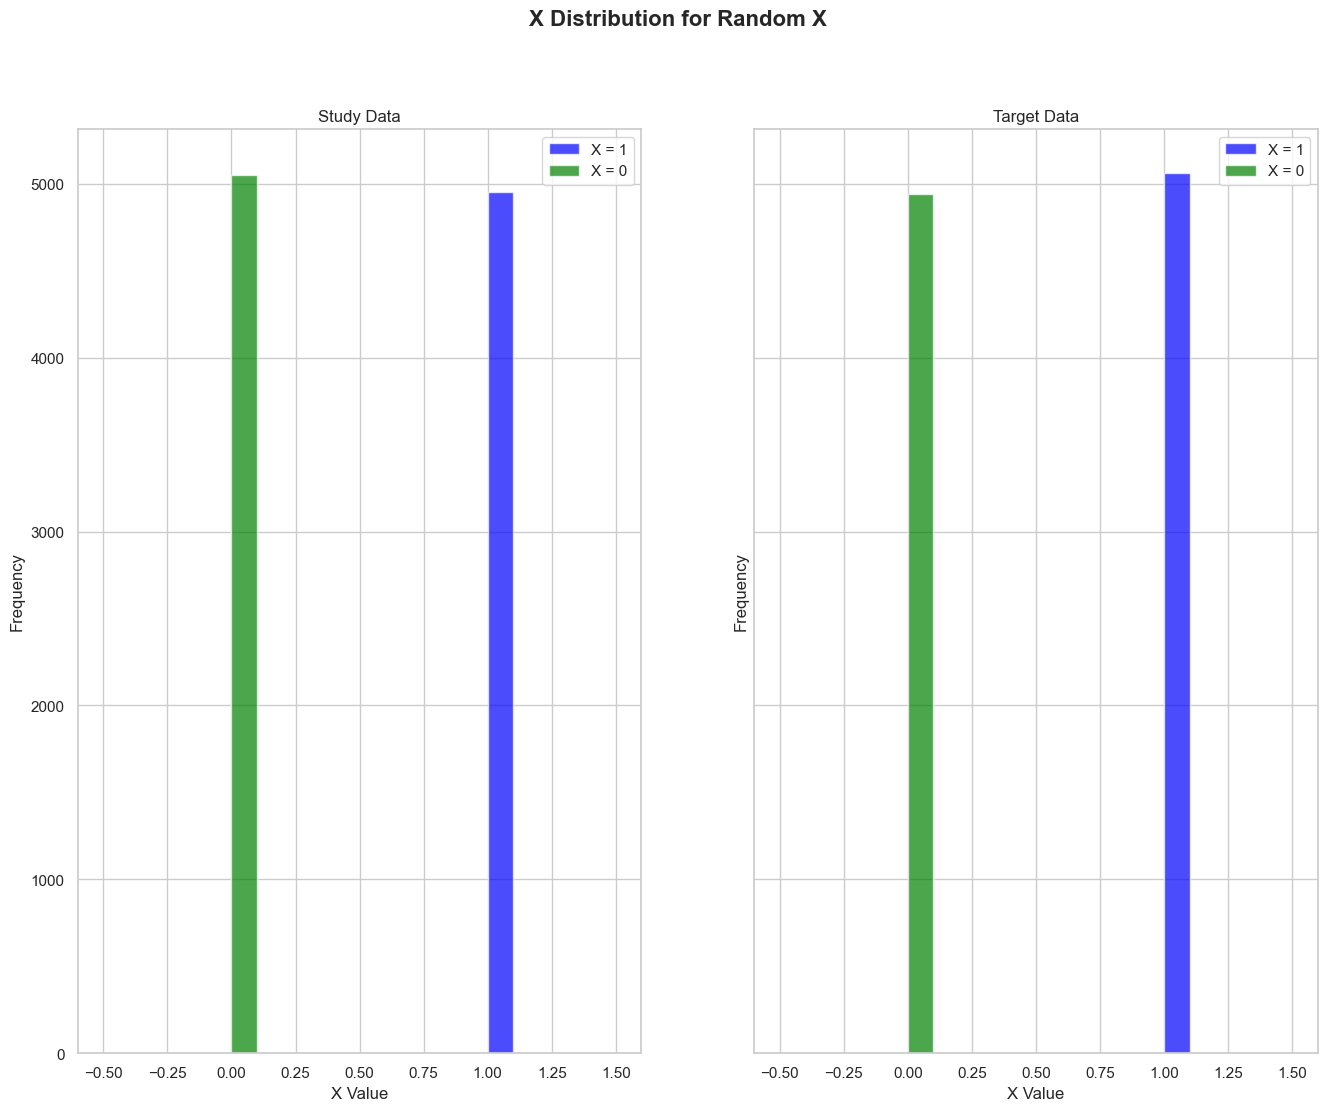
\includegraphics[width=0.5\linewidth]{Report/Figure/xrandom.jpg}
    \caption{The histogram shows the distribution of $X=1$ and $X=0$ in the study and target data in the first simulation scenario, where $X$ is randomly assigned. The left panel represents the study data, while the right panel represents the target data.}
    \label{fig:xrandom}
\end{figure}

\begin{table}[!h]
\centering
    \tiny
    \begin{tabular}{|c|c|c|}
        \toprule
    Left-aligned & Centered & Right-aligned \\ 
        \midrule
    Dataset & Mean & Std \\ 
    Study Data & 0.496 & 0.25 \\ 
    target Data & 0.506 & 0.25 \\ 
    \bottomrule
    \end{tabular}
    \caption{The table represents the mean and standard deviation of $X$ in the study and target data when $X$ is randomly assigned in both datasets. The values are rounded to $3$ decimal places.}
    \label{tab:x_random}

\end{table}



\begin{figure}[!h]
    \centering
    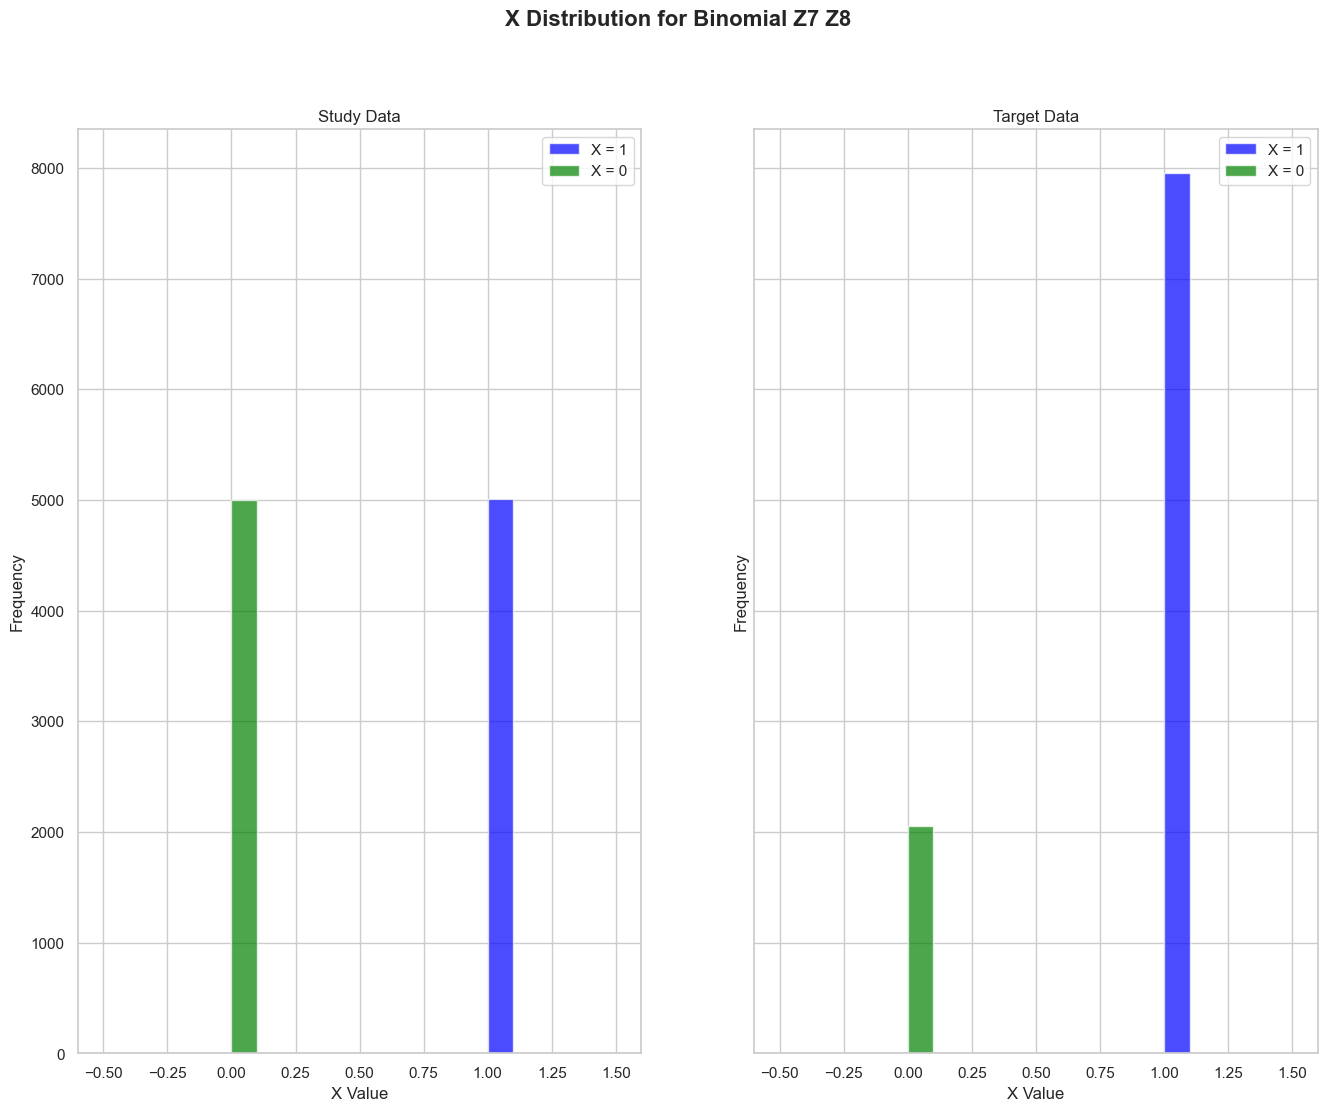
\includegraphics[width=0.5\textwidth]{Report/Figure/xnorandom1.jpg}
    \caption{The histogram shows the distribution of $X=1$ and $X=0$ in the study and target data for the second simulation scenario, where $P(X)$ in the target data is determined by $Z_7$ and $Z_8$, which are binomially distributed. The left panel represents the study data, while the right panel represents the target data.}
    \label{fig:xnorandom1}
\end{figure}

\begin{table}[!h]
\centering
\tiny
\begin{tabular}{|c|c|c|}
    \toprule
    Left-aligned & Centered & Right-aligned \\ 
    \midrule
    Dataset & Mean & Std \\ 
    Study Data & 0.501& 0.25 \\ 
    target Data & 0.795 & 0.163 \\ 
    \bottomrule
\end{tabular}
\caption{The table represents the mean and standard deviation of $X$ in the study and target data when $X$ is not randomly assigned in the target data. The values are rounded to $3$ decimal places. In this case, $P(X)$ in the target data depends on $Z_7$ and $Z_8$. $Z_7$ and $Z_8$ follow binomial distributions.}
\label{tab:x_z7z8_bi}
\end{table}


\begin{figure}[!h]
    \centering
    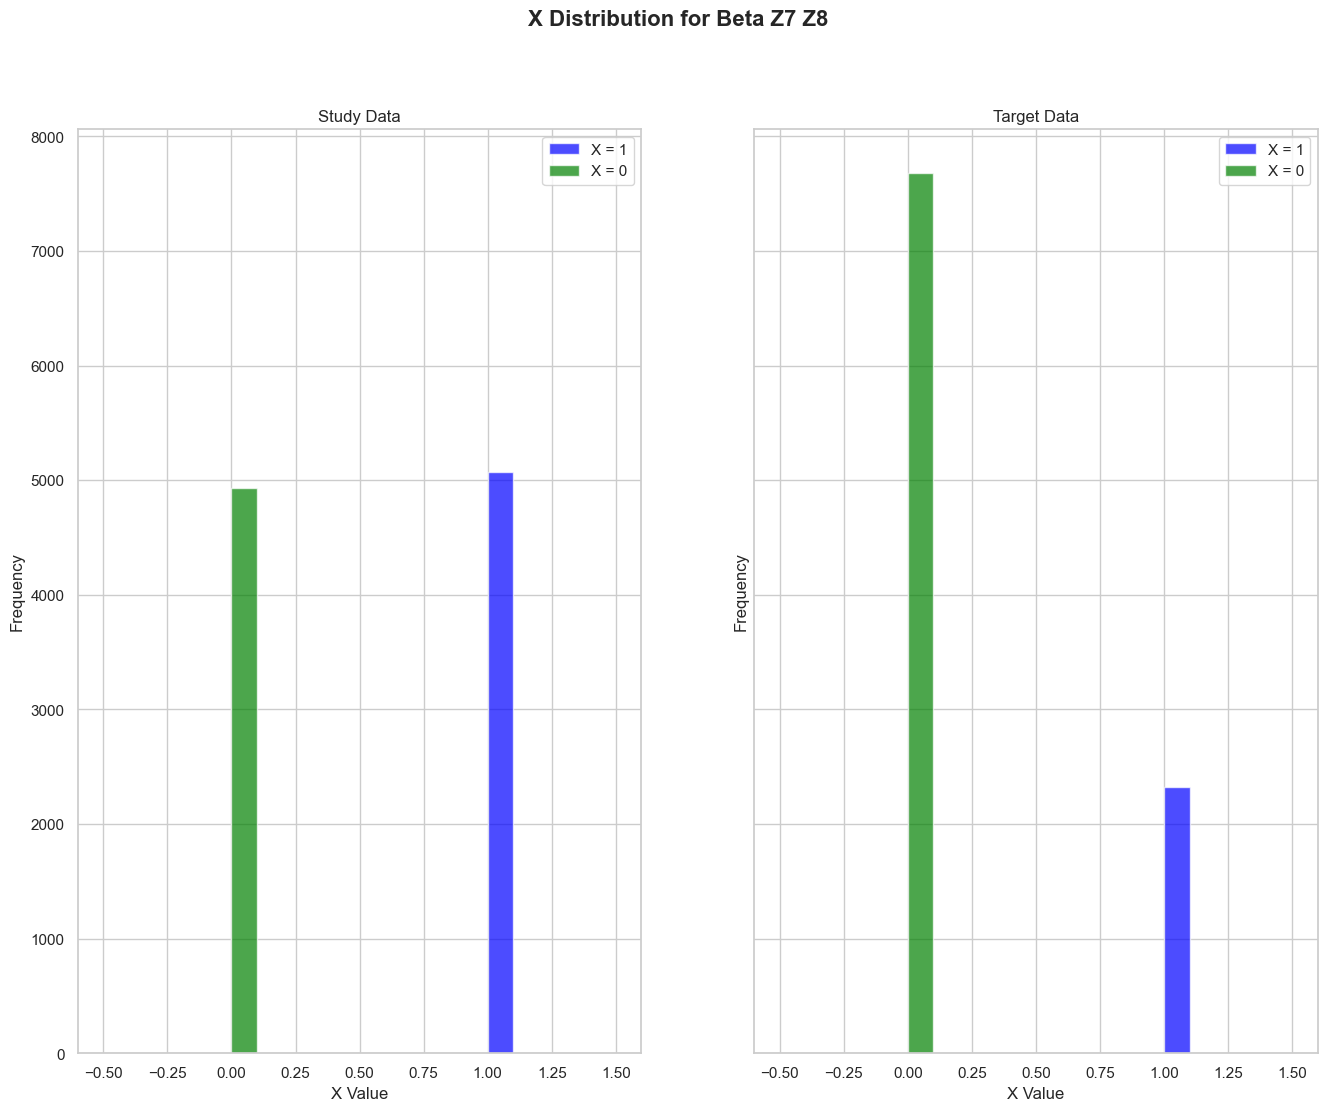
\includegraphics[width=0.5\textwidth]{Report/Figure/xnorandom2.jpg}
    \caption{Distribution of $X=1$ and $X=0$ in the study and target data for the third simulation scenario, where $P(X)$ in the target data is determined by $Z_7$ and $Z_8$, which follows beta distribution. The left panel represents the study data, while the right panel represents the target data.}
    \label{fig:xnorandom2}
\end{figure}

\begin{table}[!h]
\centering

\tiny
\begin{tabular}{|c|c|c|}
    \toprule
    Left-aligned & Centered & Right-aligned \\ 
    \midrule
    Dataset & Mean & Std \\ 
    Study Data & 0.507 & 0.25 \\ 
    target Data & 0.232 & 0.178 \\ 
    \bottomrule
\end{tabular}
\caption{The table represents the mean and standard deviation of treatment assignment $X$ in study data and target data when $X$ is not randomly assigned in the target data. The values are rounded to $3$ decimal places In this case, $P(X)$ in the target data depends on $Z_7$ and $Z_8$. $Z_7$ and $Z_8$ follows beta distributions.}
\label{tab:x_z7z8_be}
\end{table}


Across all simulations, $Z_3$ and $Z_6$ are treated as effect modifiers (EMMs), but only $Z_6$ differs in distribution between the study and target populations. We estimate RD using three modeling approaches: (1) outcome models without interaction terms, (2) models including only the $X \times Z_6$ interaction, and (3) models including interaction terms $X \times Z_3$ and $X \times Z_6$. Linear terms for covariates involved in interactions are always included in models containing interaction terms to ensure correct model specification and proper interpretation of the interaction effects. For example, if the model only interacts with $Z_6$, there is always a linear $Z_6$ term. If the model interacts with $Z_6$ and $Z_3$, there are always a linear $Z_6$ term and a linear $Z_3$ term. 

In all three approaches, we use different combinations of linear terms involving the non-EMMs (i.e., $Z_1$, $Z_2$, ... $Z_8$) to testify how those variable selections would affect estimating RD. We followed the original paper in using stratified models for $X$ (separate models for treated and untreated groups) when no interaction terms are involved; however, when interaction terms are included, we instead fit a single joint model that included $X$, selected covariates, and interaction terms.


\subsection{Simulation Results}
To assess the performance of different modeling strategies, we present:
\begin{itemize}
    \item \textbf{Three tables} (Figures \ref{fig:om}--\ref{fig:om_xz3z6}) summarizing the mean, standard deviation (Std), and mean squared error (MSE) of RD estimates across $500$ simulations. These results compare models with and without interaction terms under three different data-generating processes (DGPs) for $X$ and $Z_7$, $Z_8$.
    \item \textbf{Two sets of line plots} (Figures \ref{fig:line_mse} and \ref{fig:line_std}), visualizing how MSE and Std vary across models. These plots contrast linear models (without interaction terms) that include the crucial EMM $Z_6$ against models incorporating interaction terms.
\end{itemize}
We aim to explore on three naturally raised questions: How does \textbf{random vs. non-random treatment assignment} affect RD estimates? Do \textbf{interaction terms} improve or worsen the estimate in terms of MSE and Std of the estimates? What is the \textbf{best modeling strategy} based on the results?
\\

\textbf{Impact of Random vs. Non-Random Treatment Assignment.}
Our results suggest that whether treatment assignment in the target population is random or not does not make a major difference in RD estimation, as long as the key effect measure modifier (EMM) \( Z_6 \) is included in the model. When \( Z_6 \) is omitted, we see a slight improvement in MSE under random exposure assignment. However, once \( Z_6 \) is included—either as a linear term or as an interaction term with \( X \)—this advantage disappears, though the standard deviation remains slightly lower when \( X \) is randomly assigned. The results are presented in Figures \ref{fig:om}
to \ref{fig:om_xz3z6}. 

One possible explanation is that when the correct covariates are included, the model already accounts for systematic differences in exposure assignment between the study and target populations, making randomization in treatment assignment less important for RD estimation.

Overall, while random exposure assignment may provide a small advantage in standard deviation when the main EMM is included, its overall impact on RD estimation appears minimal. This suggests that careful covariate selection might be more important than the specific exposure assignment mechanism when generalizing causal effects.




\begin{figure}[h]
    \centering
    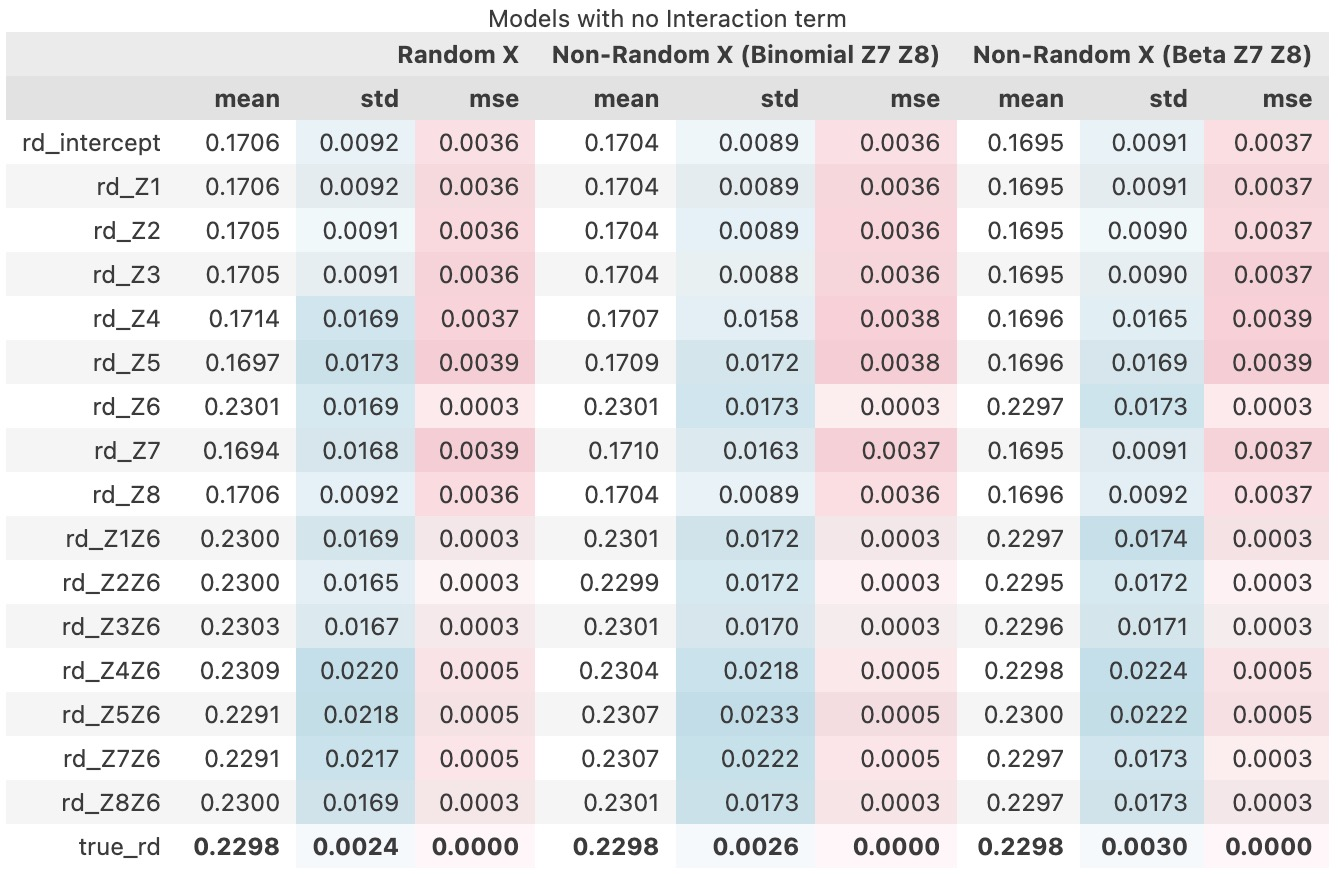
\includegraphics[scale=0.22]{Report/Figure/om.jpg}
    \caption{Results for models without interaction terms, comparing random and non-random treatment assignment across three simulation settings introduced earlier. The first three columns correspond to Simulation 1, the middle three to Simulation 2, and the right three to Simulation 3. Notation Pattern: \textit{rd\_intercept} represents a model with only the intercept and $X$, \textit{rd\_Z1} includes the intercept, $X$, and $Z_1$, and \textit{rd\_Z1Z6} includes the intercept, $X$, $Z_1$, and $Z_6$. \textit{true\_rd} is the RD calculated from the target population data. Lighter colors indicate lower bias and variance, while darker colors indicate higher values, reflecting model stability and performance.}
    \label{fig:om}
\end{figure}

\begin{figure}[h]
    \centering
    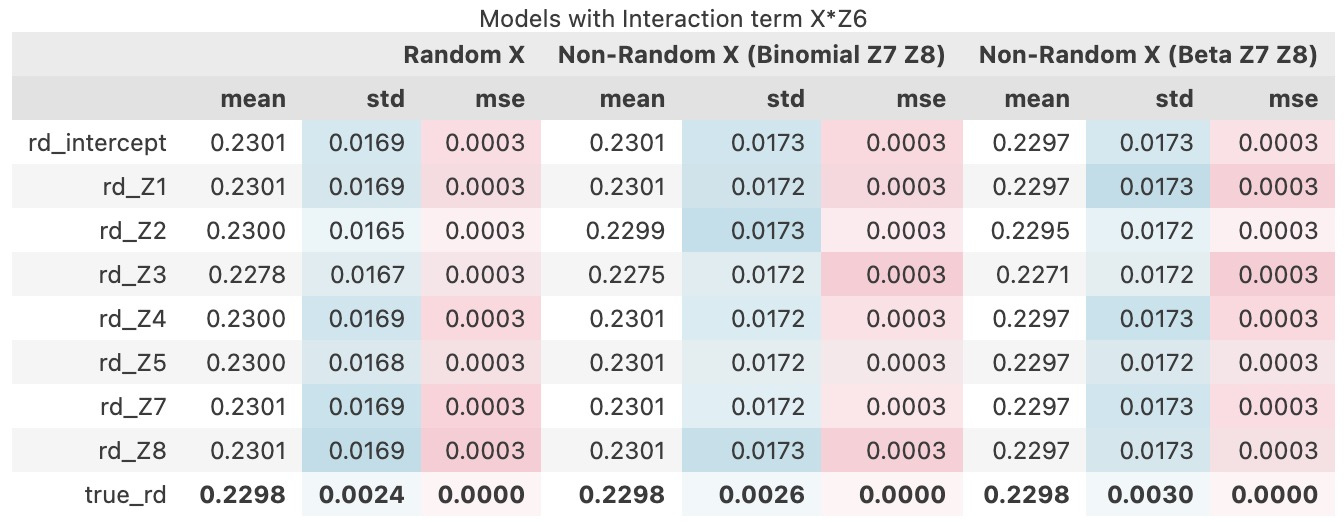
\includegraphics[scale=0.22]{Report/Figure/om_xz6.jpg}
    \caption{Results for models including the interaction term $X \times Z_6$, comparing random and non-random treatment assignment across three simulation settings introduced earlier. The first three columns correspond to Simulation 1, the middle three to Simulation 2, and the right three to Simulation 3. Notation Pattern: \textit{rd\_intercept} represents a model including the interaction term $X \times Z_6$, the linear term $Z_6$, the intercept, and $X$. \textit{rd\_Z1} includes the same components as \textit{rd\_intercept}, plus the linear term $Z_1$. \textit{true\_rd} is the RD calculated from the target population data. Lighter colors indicate lower bias and variance, while darker colors indicate higher values, reflecting model stability and performance.}
    \label{fig:om_xz6}
\end{figure}

\begin{figure}[h]
    \centering
    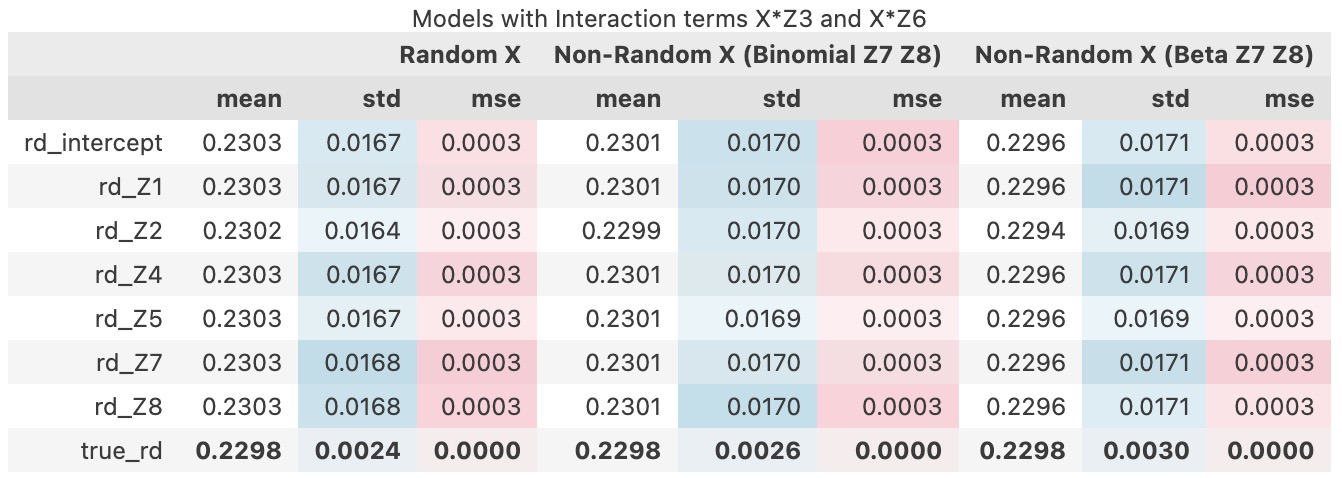
\includegraphics[scale=0.22]{Report/Figure/om_xz3z6.jpg}
    \caption{Results for models including the interaction terms $X \times Z_6$ and $X \times Z_3$, comparing random and non-random treatment assignment across three simulation settings introduced earlier. The first three columns correspond to Simulation 1, the middle three to Simulation 2, and the right three to Simulation 3. Notation Pattern: \textit{rd\_intercept} represents a model including the interaction terms $X \times Z_6$ and $X \times Z_3$, the linear terms $Z_6$ and $Z_3$, the intercept, and $X$. \textit{rd\_Z1} includes the same components as \textit{rd\_intercept}, plus the linear term $Z_1$. \textit{true\_rd} is the RD calculated from the target population data. Lighter colors indicate lower bias and variance, while darker colors indicate higher values, reflecting model stability and performance.}
    \label{fig:om_xz3z6}
\end{figure}


\textbf{Effect of Interaction Terms on Estimation Stability.} 
We find that including interaction terms for EMMs slightly reduces variance compared to including an EMM as only a linear term. A possible explanation is that modeling a strong effect modifier as an interaction term can help reduce residual (unexplained) variation, which \textbf{offsets} the variance cost of estimating an additional parameter, leading to more stable estimates.

However, the overall improvement in MSE is minimal, as models that include the crucial EMM as a linear term already exhibit low MSE. This suggests that, in the current simulation setting, omitting interaction effects does not induce substantial bias in RD estimation. Nonetheless, we observe that when interaction terms are omitted but non-EMMs (\( Z_4 \), \( Z_5 \), and \( Z_7 \)) are included, both MSE and Std increase noticeably. Since these variables differ between the study and target populations, their inclusion without modeling interaction effects may introduce instability in RD estimation. Results are presented in Figures \ref{fig:line_mse} and \ref{fig:line_std}. 

Comparing models that include only \( X \times Z_6 \) versus those that include both \( X \times Z_3 \) and \( X \times Z_6 \), we find no meaningful difference in MSE. However, models incorporating both interaction terms exhibit lower Std. This suggests that while adding \( X \times Z_3 \) does not substantially alter the expected risk difference, it may help stabilize estimation by better capturing treatment effect heterogeneity.

 



\begin{figure}[h]
    \centering
    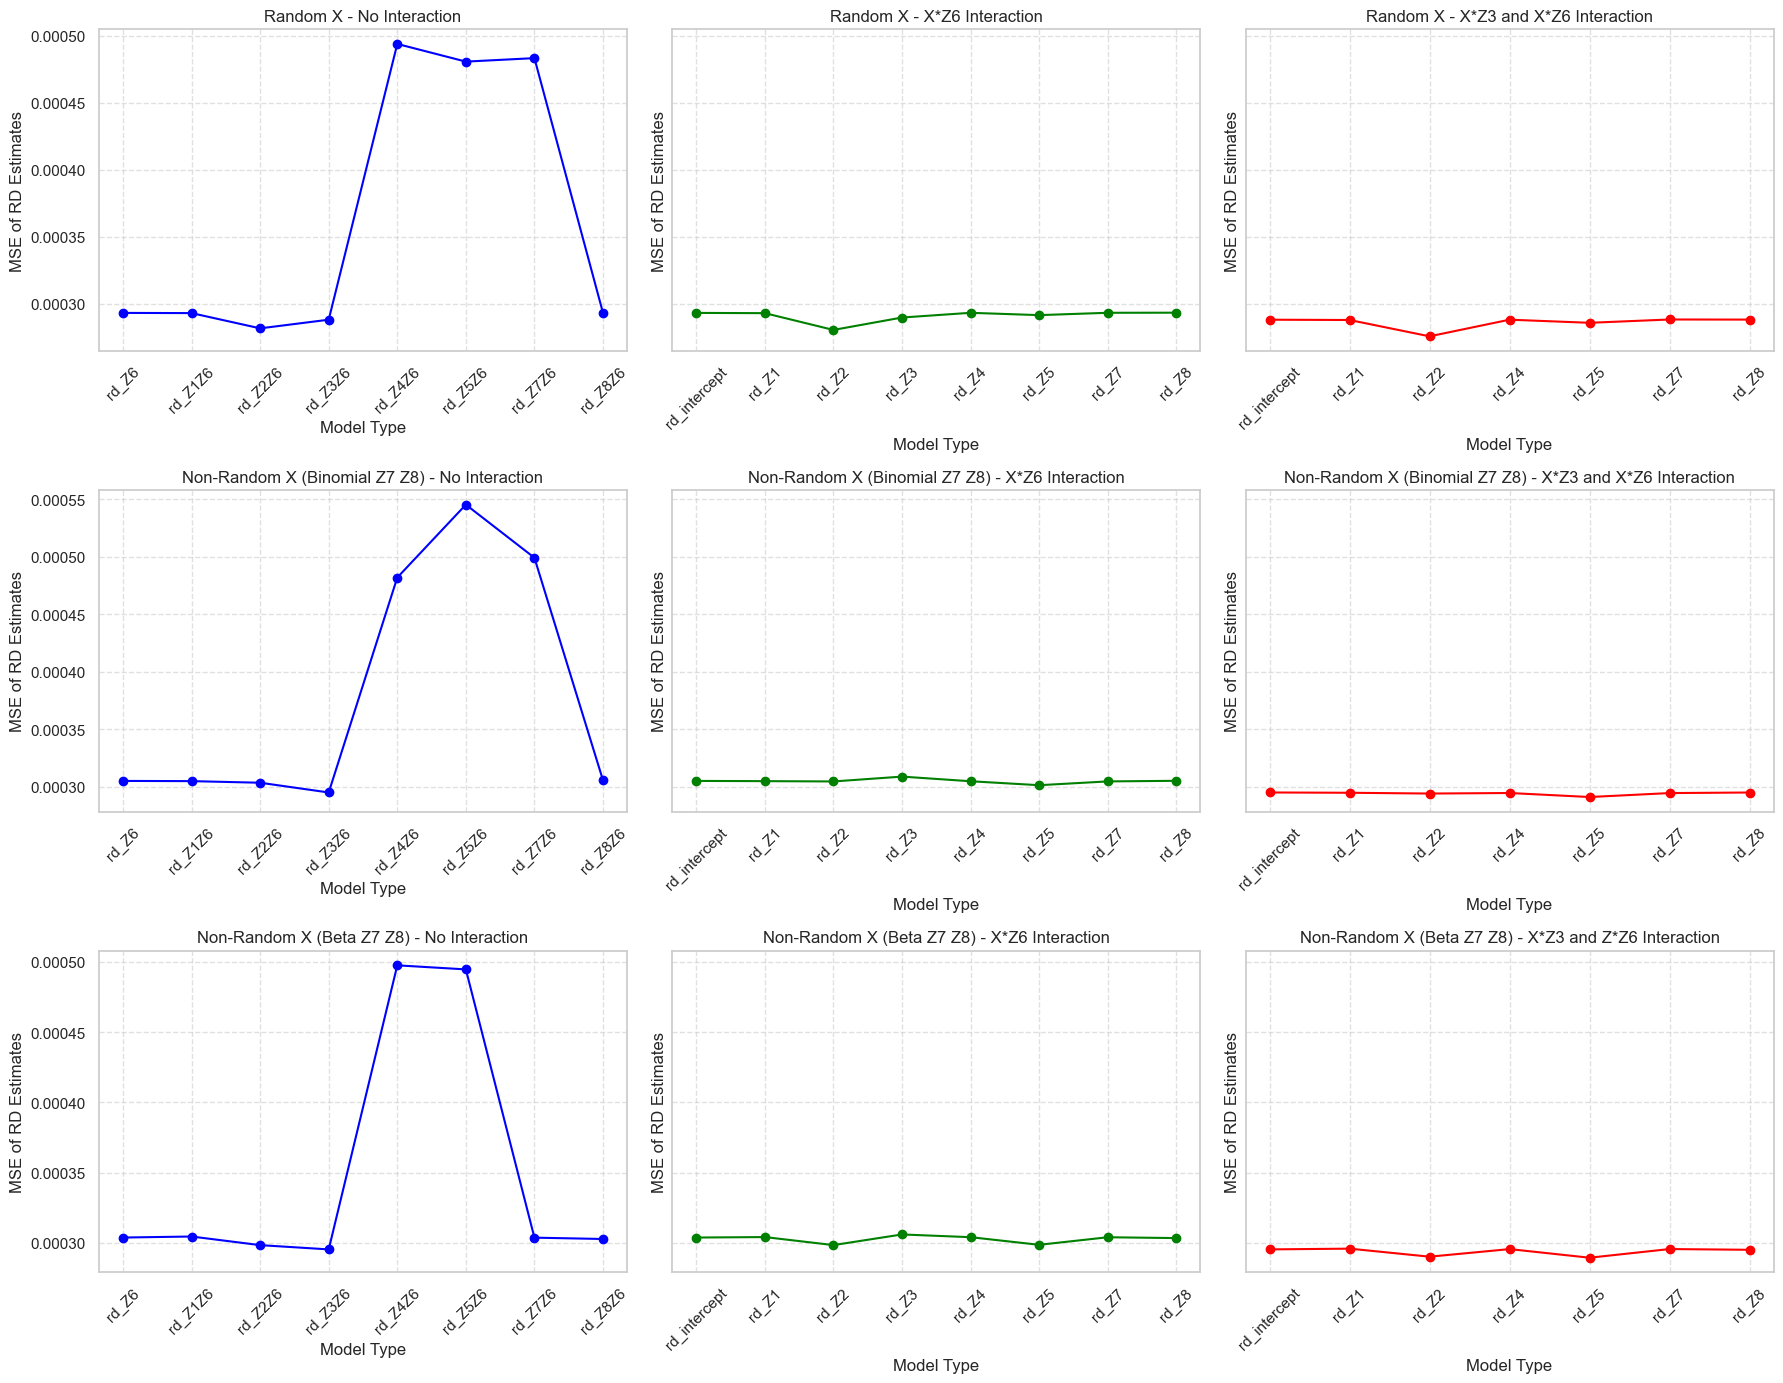
\includegraphics[width=0.9\linewidth]{Report/Figure/line_mse.jpg}
    \caption{Line plots of Mean Squared Error (MSE) in the RD estimates under different model specifications. The first column shows models without interaction terms, the second column includes models with the interaction term $X \times Z_6$, and the third column incorporates both $X \times Z_3$ and $X \times Z_6$. The first row represents scenarios where $X$ is randomly assigned in the target population, while the second and third rows correspond to non-random treatment assignment with different distributions of $Z_7$ and $Z_8$ influencing $X$.}
    \label{fig:line_mse}
\end{figure}

\begin{figure}[h]
    \centering
    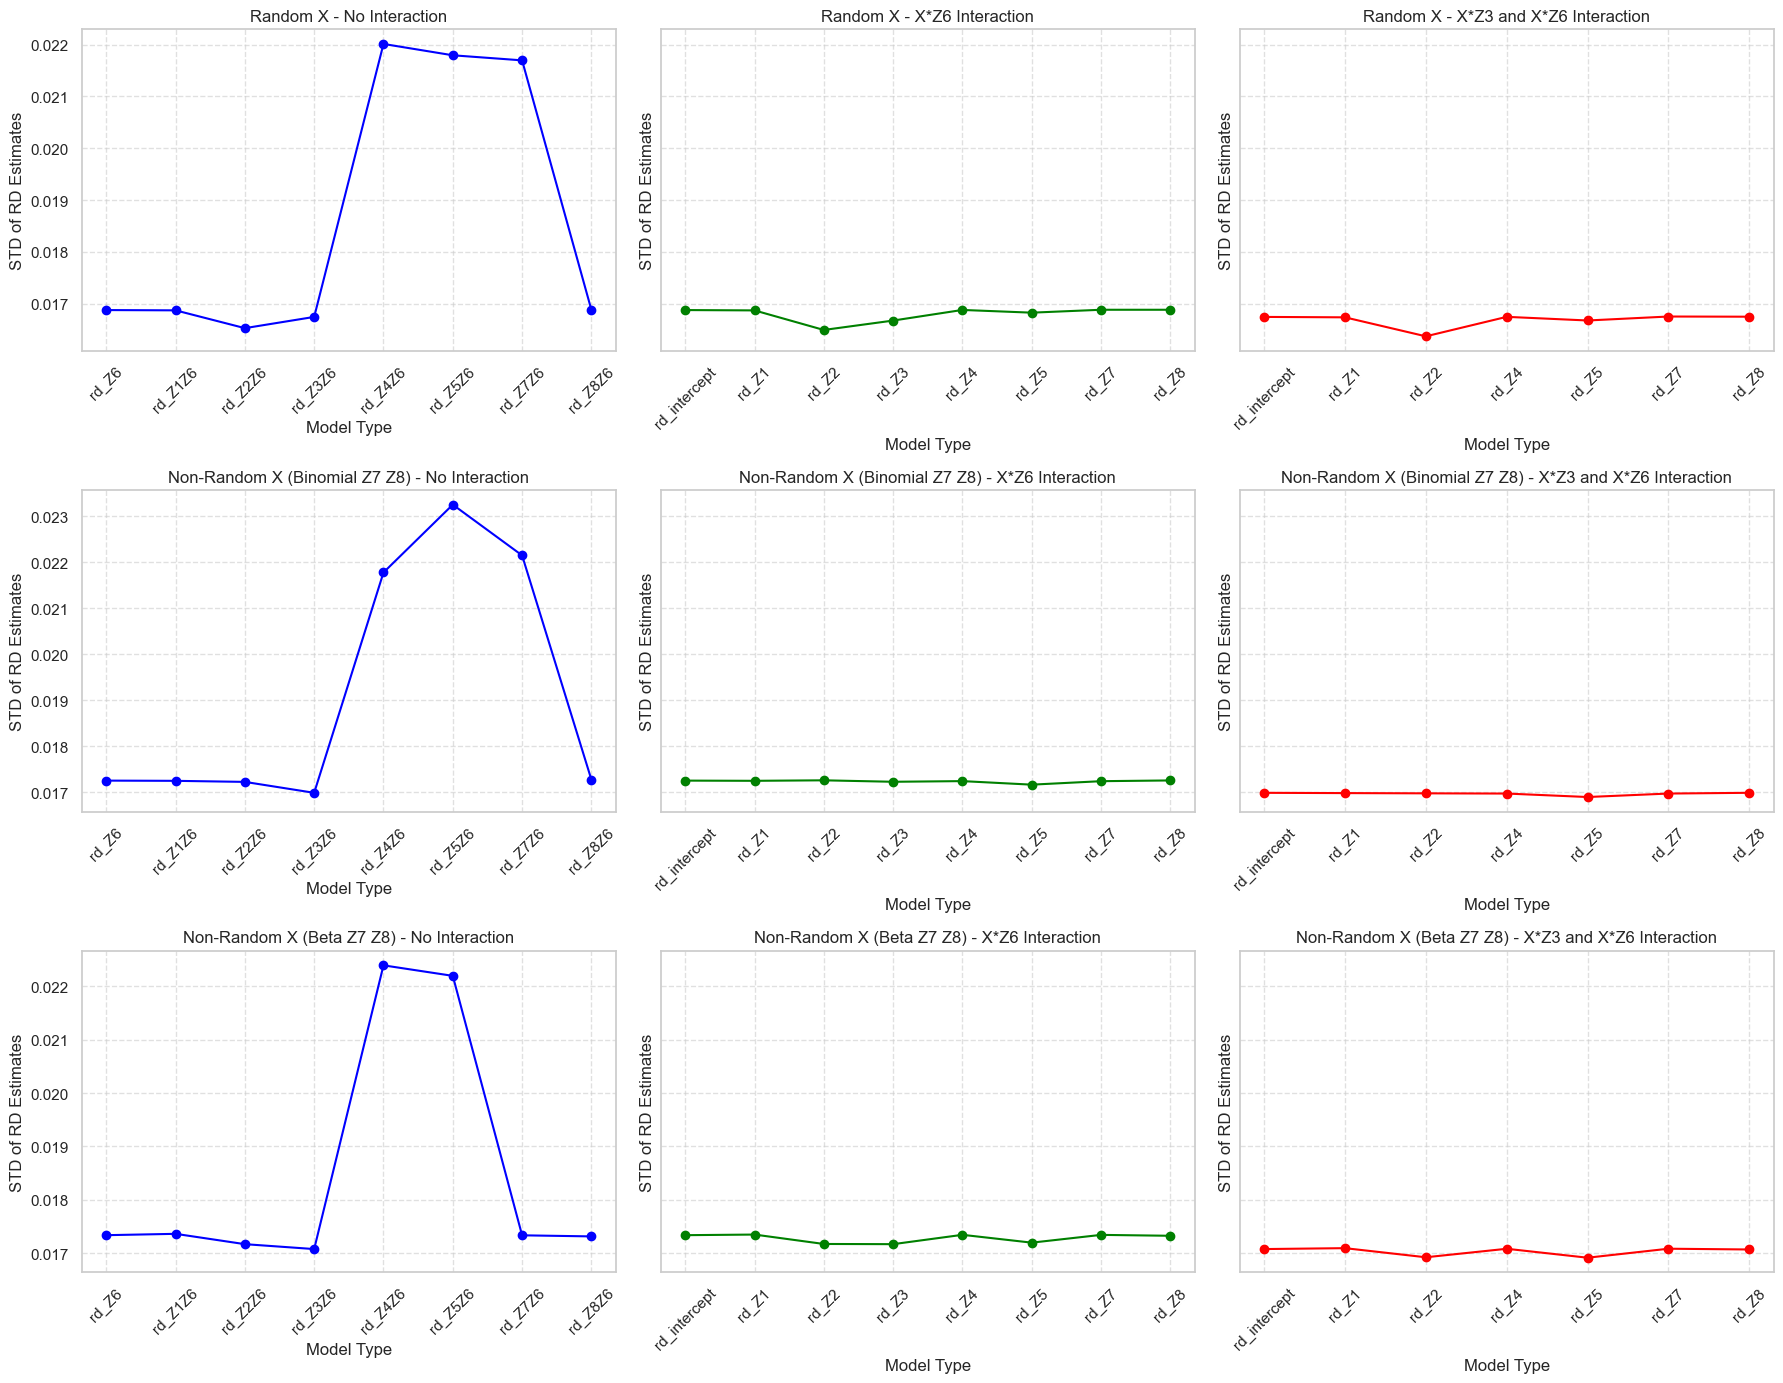
\includegraphics[width=0.9\linewidth]{Report/Figure/line_std.jpg}
    \caption{Line plots of Standard Deviation (Std) in the RD estimates under different model specifications. The first column shows models without interaction terms, the second column includes models with the interaction term $X \times Z_6$, and the third column incorporates both $X \times Z_3$ and $X \times Z_6$. The first row represents scenarios where $X$ is randomly assigned in the target population, while the second and third rows correspond to non-random treatment assignment with different distributions of $Z_7$ and $Z_8$ influencing $X$.}
    \label{fig:line_std}
\end{figure}


\textbf{Best modeling strategy.} Based on our results, it is recommended that:

\begin{enumerate}
    \item Always include the key EMM $Z_6$ to prevent bias.
    \item Including EMMs (even if they do not differ across populations, like $Z_3$) \textbf{reduces variance} in the estimates, leading to \textbf{more stable and precise RD estimates}.
    \item \textbf{Preferably} include EMMs as interaction terms when there is theoretical justification or empirical evidence supporting their role in the true data-generating process.
    \item Avoid including non-EMMs that differ across populations unless necessary, as they may increase variance without reducing bias.
    \item If non-EMMs must be included, ensure that interactions involving key EMMs are also modeled to mitigate variance inflation.
\end{enumerate}
This strategy aims to balance bias reduction and variance stability, leading to the most reliable RD estimates in external validity settings.


\subsection{Conclusion}  
Our findings align with the original paper’s conclusion that essential effect measure modifiers (EMMs)—particularly those differing between study and target populations—need to be included for unbiased RD estimate and including non-EMMs differ between populations decreases precision but does not amplify bias. While adding interaction terms does not substantially improve risk difference (RD) estimation in our simulations, this may be due to the simplicity of our experimental setup. A more realistic scenario could involve varying the magnitude of interactions or incorporating more complex structures—such as higher-order or nonlinear effects—to test the robustness of variable selection strategies. 

Additionally, future studies should explore more complex modeling settings beyond interaction terms. Introducing selection bias, unmeasured confounding, or nonlinear dependencies could better reflect real-world transportability challenges. Since our results indicate minimal gains from including interactions under the current setup, further research should assess whether a more sophisticated experimental design would show more distinct results.

Importantly, \textbf{identifying EMMs} in real-world data is challenging. As the original paper also emphasizes, prioritizing variables strongly associated with the outcome is often a reasonable approach, even if it comes at the cost of increased variance. This highlights an inherent bias-variance trade-off in selecting adjustment sets for external validity. 




\clearpage
\printbibliography
\end{document}
